\chapter{Instalación}
Para la instalación de ERP5 nos hemos de ir a la página oficial www.erp5.com y pulsar sobre download donde se nos mostrarán las posibles opciones de descarga. En este caso, vamos a escoger la segunda que es la de la máquina virtual, pues el SO sobre el que estamos haciendo la instalación es Manjaro, una distribución de Arch Linux que no tiene soporte para el ERP. 
Hacemos click sobre “how to setup a virtual machine running ERP5”

Antes de instalar nos debemos de asegurar que cumplimos todos los requisitos indicados:
\begin{itemize}
	\item Tener instalado VMWare(ya que ERP5 para VM está en formato vmx)
	\item 7 GB de espacio en disco
	\item 2 GB de RAM
\end{itemize}

Hacemos click sobre el enlace de descarga que nos redireccionará a una página donde se nos abrirá una descarga automática:

\begin{figure}[!h]
  \centering
    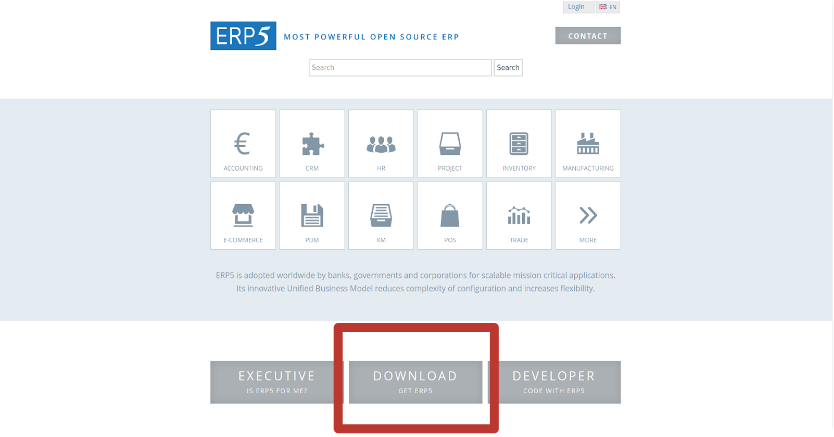
\includegraphics[scale=0.5]{descarga.png}
\end{figure}

Abrimos la máquina virtual y pulsamos sobre “Open Virtual Machine” y escogemos el archivo descargado anteriormente. Escogemos “ERP5 Release”. Ahora se nos pedirán unas credenciales, que podemos encontrar en la guía de instalación de la página oficial de ERP5:
\begin{itemize}
	\item Usuario: tux
	\item Contraseña: linux
\end{itemize}

\begin{figure}[!h]
  \centering
    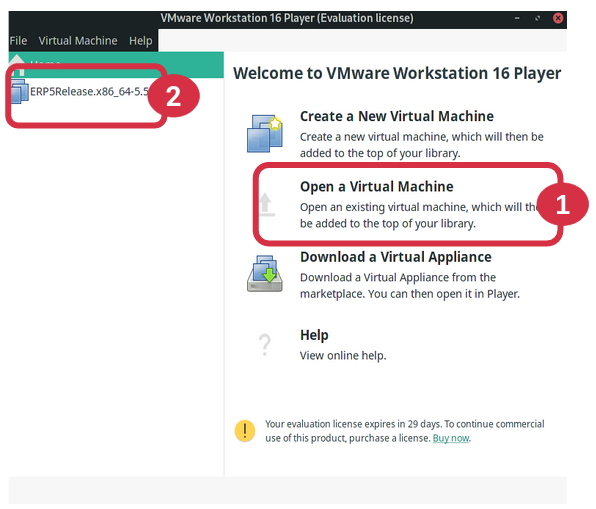
\includegraphics[scale=0.5]{conf.png}
\end{figure}

\begin{figure}[!h]
  \centering
    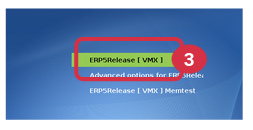
\includegraphics[scale=0.5]{erp.png}
\end{figure}

Una vez logueados se nos abrirá directamente el navegador con ERP5. Volvemos a introducir las mismas credenciales. Una vez iniciado sesión vemos la página principal de ERP5 donde se muestran los distintos modos con los que cuenta

